\documentclass[12pt, orivec, fleqn]{article}
\usepackage[no-math]{fontspec}
\usepackage{amsmath}
\usepackage{amssymb}    % for \rightsquigarrow
\usepackage{wasysym}	% for frown face
\usepackage[most]{tcolorbox}
\usepackage{ulem}
\usepackage{tikz-cd}	% commutative diagrams
\usepackage{tikz}
\usepackage{amsthm}
\usepackage{enumitem}	% for \itemize custom labels
\usepackage{turnstile}	% longer turnstiles

\usepackage{hyperref}
\usepackage{minitoc}

\usepackage[sf,bf,big,raggedright,compact]{titlesec}	% change section color to blue
\usepackage[backend=biber,bibstyle=authoryear]{biblatex}
\bibliography{../AGI-book}

\ifdefined\chinchin
	\setromanfont{AlibabaSans-Light.otf}
	\usepackage[CJKspace]{xeCJK}
	\setCJKmainfont[FallBack, BoldFont=Alibaba-PuHuiTi-Regular.ttf, ItalicFont=Alibaba-PuHuiTi-Medium.ttf]{Alibaba-PuHuiTi-Light.ttf}
	\newcommand{\cc}[2]{#1}
\else
	\setromanfont{Ubuntu}
	\newcommand{\cc}[2]{#2}
\fi

\newtheorem{theorem}{Theorem}

\setcounter{secnumdepth}{2}		% 0 = no section numbers

\titleformat{\section}[hang]{\Large\color{blue}}{\thesection \hspace{10pt}}{0pt}{}
\titleformat{\subsection}[hang]{\large\color{blue}}{\thesubsection \hspace{5pt}}{0pt}{}

\newcommand{\book}[1]{$\NewSym[0.4]{../book-icon.png} \quad$ \parbox{0.9\textwidth}{\footnotesize #1}}
\newcommand{\code}[1]{{\footnotesize{\ttfamily #1}}}
\newcommand{\tab}{\hspace*{2cm}}
\newcommand{\powerset}{\raisebox{.15\baselineskip}{\Large\ensuremath{\wp}}}
\newcommand{\Chi}{\raisebox{2.5pt}{$\chi$}}
\newcommand*\KB{\vcenter{\hbox{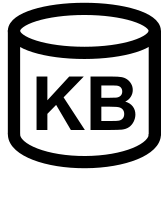
\includegraphics{../KB-symbol.png}}}}
\newcommand*\NewSym[2][0.5]{\vcenter{\hbox{\includegraphics[scale=#1]{#2}}}}
\newcommand*\sigmoid{\vcenter{\hbox{
\includegraphics{sigmoid.png}}}}
\newcommand{\smbox}[1]{\boxed{\footnotesize{\mbox{#1}}}}

\newcommand{\tikzmark}[1]{\tikz[overlay,remember picture] \node (#1) {};}

\newcommand{\Dfrac}[2]{%
	\ooalign{%
		$\genfrac{}{}{2.9pt}0{\hphantom{#1}}{\hphantom{#2}}$\cr%
		$\color{white}\genfrac{}{}{1.5pt}0{\hphantom{#1}}{\hphantom{#2}}$\cr%
		$\color{white}\genfrac{}{}{1pt}0{\color{black}#1}{\color{black}#2}$}}

\renewcommand{\thefootnote}{\fnsymbol{footnote}}
\interfootnotelinepenalty=10000

\addtolength{\oddsidemargin}{-1in}
\addtolength{\evensidemargin}{-1in}
\addtolength{\textwidth}{2in}

\title{$\hbox{
\includegraphics[scale=2]{COCO-logo.png}}$ \\
	\vspace*{0.5em}
	\color{blue} COCO white paper}
% \author{\cc{甄景贤}{YKY}}

\begin{document}
\setlength{\parindent}{0pt}
\setlength{\parskip}{2.8ex plus0.8ex minus0.8ex}

\maketitle

\begin{abstract}
COCO is a decentralized, autonomous, anonymous / named, open-source, for-profit, platform for online collaborative projects based on virtual shares.
\end{abstract}

\dosecttoc
\tableofcontents

\secttoc
\section{\cc{問題的背景}{Background of the problem}}

\begin{itemize}
	\item \cc{我是一个从小时候(80年代初)开始玩电脑的人,亲身经历了 programmer / hacker 文化的演变过程}
	{I first got in touch with computers in the early 1980's, witnessed the growth and change of the programmer / hacker culture}
	
	\item \cc{写程式是一件很有趣的,creative 的过程}
	{Writing code is a fascinating, creative process}
	
	\item \cc{但后来出现了 Windows 的 收费/闭源 和 Linux 免费/开源 的对立}
	{Then came the split between proprietary Windows versus open-source Linux}
	
	\item \cc{Open source 软件的 \textbf{奖励机制} 一直很有问题,开发者基本上抱著「无偿奉献」的心态,很难获得和付出成比例的回报}
	{From the beginnning, open source has lacked a good \textbf{reward mechanism}, developers have to make ``selfless sacrifice'', hard to expect compensation commensurate with their efforts}
	
	\item \cc{最近出现了 \textbf{License Zero} 这种 for-profit open-source 软件条款,或许可以改变 open-source 不赚钱的问题}
	{Recently appeared \textbf{License Zero} which is both for-profit and open-source, perhaps can solve the problem of earning money}
\end{itemize}

\secttoc
\subsection{\cc{COCO 企图解决的问题}{What does COCO try to solve?}}

\begin{itemize}
	\item \cc{公司的\textbf{股价} 是由外在的自由市场决定(「看不见的手」)}
	{A company's \textbf{stock prices} are determined externally by the free-market (``invisible hand'')}

	\item \cc{公司内部的\textbf{股份},可以由公司自行决定,这是 COCO 企图解决的问题,希望做到比现有方法更好}
	{How the company distributes its \textbf{shares} are decided internally;  This is where COCO tries to innovate}
\end{itemize}

\secttoc
\section{\cc{实名 vs 匿名}{Real-name vs anonymous}}

\begin{itemize}
	\item All contributors are anonymous by default;  They can use their real names optionally
	
	\item All contribs can be traced to their contributors;  This information can be seen publicly, although the identity of the contributor may be unknown
\end{itemize}

\secttoc
\subsection{\cc{知识产权的特点}{Uniqueness of intellectual properties}}

We decide to adopt an \textbf{anonymous} policy because:
\begin{itemize}
	\item Contribs are creative, informational items that can be easily recognized (seems impossible to to conceal)
	\item Thus it would be easy for a contributor to disclose his authorship of the contrib, outside of our platform
	\item Once this is known, the author's friends can cast biased votes on his contrib
	\item There is no way to prevent such 'collusions' except to make all the work open to public scrutiny
	\item Whereas, by allowing anonymity, some contributors will be less likely to suffer from negative bias (such as racism or sexism)
\end{itemize}

\secttoc
\section{Shares}

\begin{itemize}
	\item Contributors get shares automatically when peers bid-vote on their \textbf{contribs}
	
	\item When an outside \textbf{investor} puts money into the company, his contrib is treated just like any other contrib.  His investment earns him an amount of shares determined by existing share-holders in the project.  This price may vary depending on the investor's outlook for the project.	
\end{itemize}

\secttoc
\section{VCS (version control system) and branching}

\begin{itemize}
	\item COCO will be built on top of a VCS (version control system) such as Git or Bazaar
	
	\item COCO provides a graphical interface to display the ``history graph'' of the project
	
	\item Each ``contrib'' in our terminology corresponds to a single or a set of commits in the VCS
	
	\item Contributors are free to create branches (alternatives)

	\item Branching occurs when there is a dispute whether to include a contrib or not

	\item After branching, all previous contribs up to that point are included in the new branch.  New contributors decide which branch they want to contribute to
\end{itemize}

\secttoc
\section{Exponential attenuation of votes}

\begin{itemize}
	\item \cc{
	根据经济学统计,财富 服从 log normal(对数正态)分布 \\
		亦即是说,财富的值「取 log 之后」服从正态分布}{
	According to economic statistics, wealth follows the \textbf{log-normal} distribution \\
	ie, the logarithm of wealth follows the normal distribution. 	
	}
		\begin{equation}
		\vcenter{\hbox{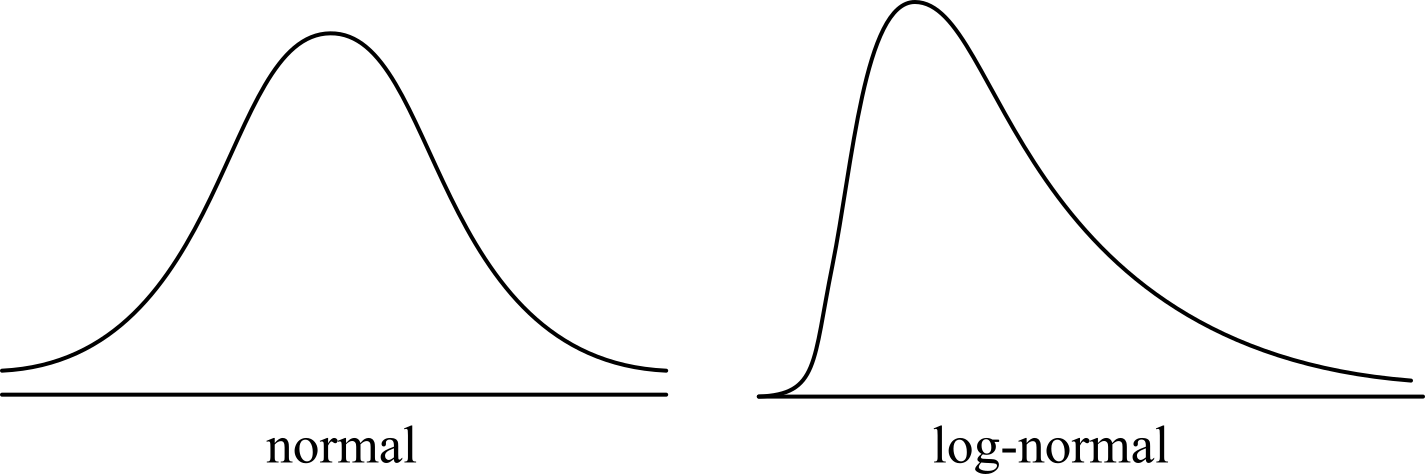
\includegraphics[scale=0.5]{normal-vs-log-normal.png}}}
		\end{equation}
	\item \cc{
	正态分布 是\textbf{对称}的(高个子与矮个子的比例相同)\\
		但财富的分布并不对称; \\
		富人的有钱程度(可能比平均值高出上万倍) \\
		远远超出穷人的贫穷程度(平均值的十分之一就是赤贫了) \\
		即财富分布曲线有右侧的长尾}{
	The normal distribution is symmetric (equal proportion of tall and short people) \\
		But the distribution of wealth is asymmetric; \\
		The wealthiest people have orders of magnitude more wealth than average. \\
		The log-normal distribution has a long tail, \\
		meaning that values far from the mean are fairly common
	}
	\item \cc{
	正态分布 形成的原因是 很多独立的因素 \textbf{相加} 而成 \\
		\textbf{对数}正态分布 则是因为 独立因素的 \textbf{相乘} 而形成}{
	The factors that contribute to a normal distribution are \textbf{additive} \\
	but the factors that contribute to a \textbf{log}-normal distribution are \textbf{multiplicative}
	}
	\item \cc{
	「成功/财富」呈 对数正态分布,\\
		原因似乎是因为 成功 导致的 positive feedback}{
	The reason why wealth or ``achievement'' is log-normal distributed \\
		seems to be due to \textbf{positive feedback}
	}	
		\footnote{
			\href{https://www.johndcook.com/blog/2009/09/29/achievement-is-log-normal/}
			{``Archievement is not Normal''}, John D Cook, 2009.
		}
	\item \cc{
	打个比方,玛莉莲梦露 在「性感」的尺度上高出平均的 1-2 个标准差  \\
		但她的粉丝的数目是 $\propto$ 当时能看到她的人口数量}{
	Let's say Marilyn Monroe's ``sexy'' measure may be 1-2 standard deviations above average \\
		but her number of fans is $\propto$ the size of the movie-going population at the time
	}
		\begin{equation}
		\vcenter{\hbox{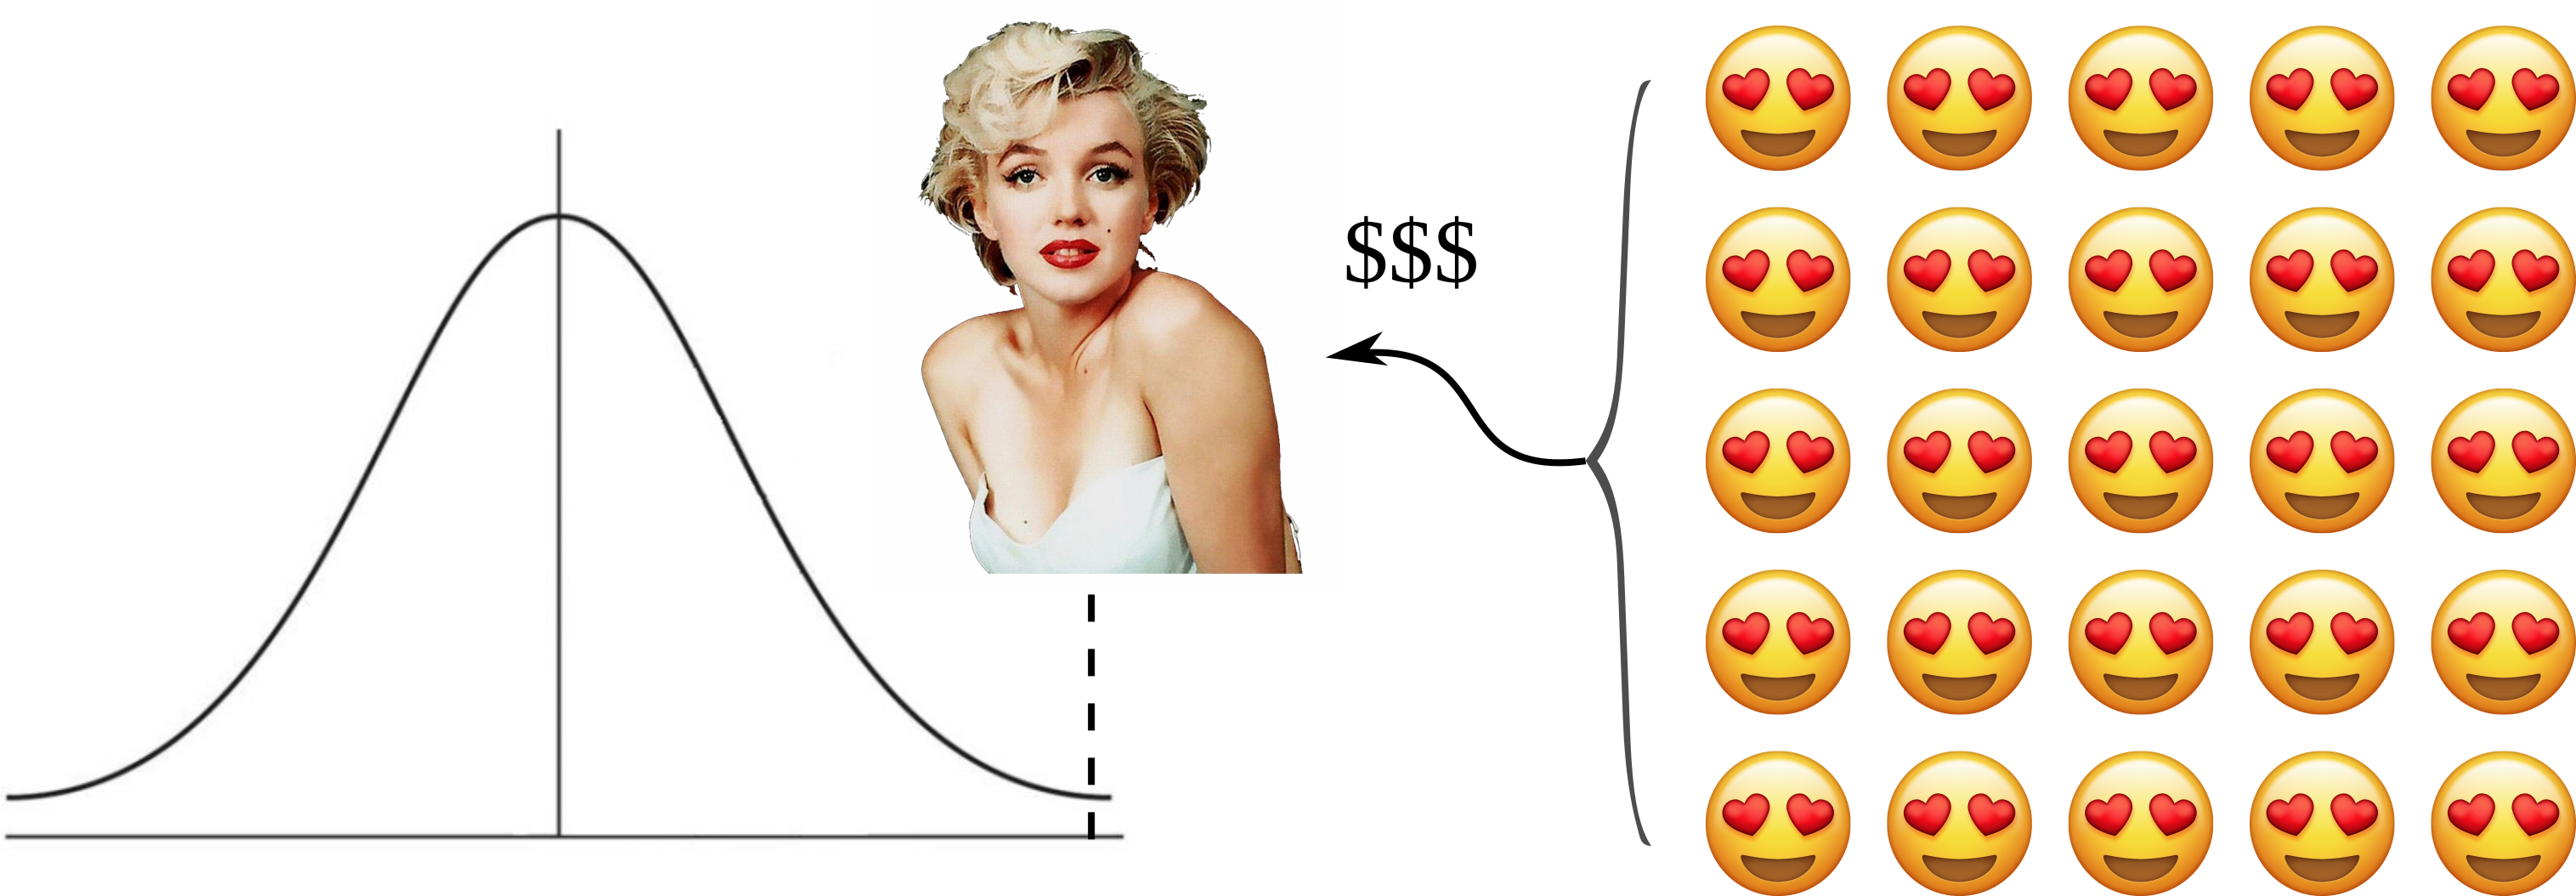
\includegraphics[scale=0.5]{exponential-voting.png}}}
		\end{equation}
	\item \cc{
	暂时我还未完全理解 财富的 positive feedback 或 exponential 效应,\\
		它大概跟上面的论述有关}{
	I have not fully understood how wealth is related to positive feedback and exponentiation \\
		but I guess the above observations may provide an explanation
	}
	\item \cc{
	我个人觉得 Coco 可以用 投票得分 的 \textbf{logarithm} 加权,这样可以导致 更平均的奖励分配,但我暂时未能给出其合理性的一个 论证....}{
	I think Coco may take the \textbf{log} of voting scores to weight shares, and this will give a more egalitarian distribution of rewards.  But I don't have a rigorous argument yet.
	}
	
\end{itemize}

\secttoc
\section{Bid-vote combination scheme}

\begin{itemize}
	\item \cc{
	我们使用一种混合 bidding 和 voting 的方法,理由是 因為 成員 在 公司 中主動貢獻的 contribs \textbf{不能收回}}{
	We consider a mixed voting-bidding scheme, the rationale being that a member's voluntary contribution cannot be \textbf{retracted}
	}
	
	\item \cc{
	如果單靠 voting 的話,貢獻者 處於被動}{
	If we rely solely on voting, contributors are in a passive position
	}

	\item \cc{
	Contributor 會比較熟悉自己貢獻的價值, which s/he claims in the bidding}{
	Contributors would be more in touch with the value of their own contributions, which s/he claims in the bidding
	}
	
	\item \cc{
	Bid 和 vote 之间的 \textbf{差异},可以表示 estimation 有没有问题,或者有争议}{
	If there is a big difference between bid and voted values, it may indicate an inaccurate assessment or a disagreement.
	}

	\item The bidding can be of the form of:
	\begin{itemize}
		\item \% shares, or
		\item cash amount
	\end{itemize}

	\item Voters can respond to the bidding by:
	\begin{itemize}
		\item agreeing
		\item disagreeing, or
		\item suggesting a new value
	\end{itemize}

	% \item Votes (also called ratings) can be any number $\in [-1,1]$.  They represent the \% (percentage shares) a user wants to give to a particular contrib.

	\item All votes are visible for public scrutiny.

	\item If some features (contribs) are seen to be voted unfairly, share-holders may initiate new branches.
\end{itemize}

\secttoc
\section{User-side voting}

\begin{itemize}
	\item This is a new feature that has never existed in traditional software products
	
	\item Users (ie, buyers of the software) are entitled to vote on features (contribs) that they like, the same as when members vote on contribs
	
	\item User input can help COCO more accurately to estimate which contribs are useful

	\item Buyers pay for the entire project, which includes all its branches / features;  They can choose to deploy any branch for usage

	\item By paying for the product, buyers automatically become share-holders;  So they have the right to up/down-vote features (contribs) just like other share-holders
\end{itemize}

\secttoc
\section{Use of AI or default values to automate voting and reduce ``voting fatique''}

Too much voting events would be detrimental to productivity.  We need to reduce the number of votings and simplify the voting process.  This can be achieved by default values either designed by humans or recommended by AI.

As to AI recommendation of default votes, we need to decide what is the objective for recommending such votes, given the AI's limited intelligence (assuming it does not yet understand users' contents).

\secttoc
\section{Potential problems and possible solutions}

\begin{itemize}
	\item ``Reputation'' may be inaccurate when members have small \# of contribs (but we focus on contribs without regard to who contributed them)
	
	\item Branching is automatic -- you don't need to care about how others vote, as long as your branch works / someone buys it
	
	\item Bad voting should be penalized, but if a contributor is already low-score, the most we can do is to reduce his score to 0.  But since each score is earned either by money or work, the penalty may still make sense.
	
	\item How to prevent the possibility of a significant contributor spawning fake contribs?  But if all the votes are visible, the significant contributor may risk losing his reputation (in the project) even if he is anonymous.
\end{itemize}

\cc{
其实 自愿 的 voting 和由此建立起的 reputation 有问题,因为 vote 别人不能带来直接的利益,而是一个 management task,传统上由 经理人 做。  但如果要取代这 management 角色,则需要一个相对地完备的机制。   Manager 接受 salary,他的工作是 control tasks, monitor work and give rewards.   问题是这件工作可不可以变成 distributive?  }{
There may be a problem with basing reputation upon voluntary votes.  Voting for someone does not benefit the voter;  This is a management task traditionally done by managers.  If we want to replace such a role, we need an adequate mechanism.  The traditional manager gets paid, and his responsibility is to control tasks, monitor work, and give rewards.  The question is whether this job can be decentralized?
}

% \pagebreak
%\footnotesize

\secttoc
\subsection{\cc{Free-riders 问题}{The problem of free-riders}}

\cc{
按道理,那些不作为的 founders,其股份应该下跌。  但怎样分辨 懒惰的 free-riders 和 要求较高的 founders?
}{
In principle, if a founder hoards shares without performing useful work, his shares in the company should be reduced.	 But how could we distinguish between lazy free-riders and someone who has high standards for other people's work?
}

\cc{
其中一个解决的可能是: 当 founders 们意见不合时可以 \textbf{分叉} (branching),....
}{
A possible solution is via \textbf{branching} when founders disagree with each other.
}

\cc{
分叉的意义是: 保留两种可能。 
}{
The essence of branching is:  to preserve both options in a disagreement.
}

\begin{enumerate}
	\item branch A accepts new contrib X
	\begin{enumerate}
		\item X is a good contrib
		\item X is a bad contrib
	\end{enumerate}
	\item branch B rejects new contrib X
	\begin{enumerate}
		\item X is a good contrib
		\item X is a bad contrib
	\end{enumerate}
\end{enumerate}

\cc{
在 (1b) 和 (2a) 的情况下,branch 1 和 branch 2 分别应该受到惩罚。
}{
In cases (1b) and (2a), branch 1 and 2 should be penalized respectively.
}

\cc{
很明显,应该有 users 能判断哪个是 better branch,但实际上可能出现 branching 太多的问题,还有 users 不能分辨有没有渗入 free-riders 的分支。 
}{
Obviously, there should exist users who can determine which branches are better, but in practice there may be too many branches to consider.  Users may be unable to tell which branches are contaminated with free-riders. 
}

\cc{
但如果所有 votes 是公开的,则在统计上,始终会是较好的 branch 胜出。 
}{
However, if all votes are openly visible, then statistically we may believe that good branches will win out eventually.	
}

\secttoc
\subsection{Insider collusion}

Typical scenario:  a sub-group of insiders systematically up-vote themselves and down-vote outsiders.  They share their identities and contribs among themselves, contrary to COCO's anonymity intention.

Solution:  If some users see their contribs are not voted fairly, they may file complaints or initiate new branches.

\cc{
首先在平台上可以查看各人投票是不是公平,如果有系统的偏差是可以侦察出来,这也是 AI 可以帮助到的,总比不记名投票好。}{
On our platform, we can examine every vote to see if they are fair.  If there is systematic bias it can be detected by people or AI algorithms.  This is definitely an improvement over secret ballot.
}

\cc{
而且公开地「结盟」本身违反了不歧视的原则,这是平台的守则不容许的,所以那些人也只能秘密进行,而这样的秘密很难大规模地维系,那已经好像阴谋论了}{
It is clearly against Coco's policy to form off-platform ``alliances'' to try to influence voting.  Such collusions can only be conducted in secret and would be hard to maintain for large numbers of people.  
}

\cc{
其实我们现代世界越来越接受不歧视各种各样的人,我觉得这趋势只会变得更好}{
	
}

We may have an additional feature to penalize bad voting?

\secttoc
\section{Calculation of shares (draft)}

Assume that \textbf{initially}, $A, B, ...$ shares the company by the ratio $A : B : ...$.  The new-comer $X$ wants to join.

We use the same symbol $A$ to denote the user as well as the ``value'' (\textbf{equity}) she owns in the company.  

Before bidding, the fraction $\frac{A}{A + B + ...}$ is the \% shares of $A$ in the company $A + B + ...$.

In practice, the equity values \uline{cannot be known internally}, we can only measure their \% percentage shares.  In other words, we always have the normalization
\begin{equation}
A + B + ... = 1
\end{equation}
and the quantities $A, B, ...$ are regarded as percentages.

The actual equity-value of these shares is \textbf{market-determined}.  This is how the traditional stock market works.

\secttoc
\subsection{Scenario 1:  New-comer $X$ offers a contrib and bids (suggests) a share amount}

Each prior member ($A$, $B$, ...) would respond with the \% percentage shares she thinks $X$ may own.  This respond is denoted $\sigma_i \in [0,1]$, from 0\% to 100\%, where $i$ is the \textbf{member index} ($A, B, ... $ etc).

The amount of shares $X$ will get is given by:
\begin{equation}
\label{shares-assigned-to-X}
\frac{X}{A + B + ...} = \sigma_A (\frac{A}{A + B + ...}) + \sigma_B (\frac{B}{A + B + ...}) + ...
\end{equation}
In other words, it is the \textbf{weighted-average} of assigned shares.

Question:  if $A$ \uline{refuses} $X$'s contrib, ie, $\sigma_A = 0$, would $A$'s original shares be \textbf{diluted}?  Under the current scheme, the answer is yes, but the dilution may be reasonable / acceptable.

\secttoc
\subsection{Scenario 2:  Prior member offers a job with a share amount}

In this case, all prior members need to collectively decide if the new-comer has accomplished the task, which is a \textbf{binary} decision (``yes'' or ``no'').

\secttoc
\subsection{After-bidding shares adjustment}

After bidding, prior members' shares must decrease to create $X$'s new shares.

The shares assigned to $X$ is given by (\ref{shares-assigned-to-X}).  So the prior members must split the \textbf{remaining} shares among themselves:
\begin{equation}
\boxed{\mbox{remainder}} \quad r = 1 - X / Z
\end{equation}
where $Z = A + B + ...$, \textit{ie}, the normalization factor.

Each prior member's shares can be renewed via this formula:
\begin{equation}
A = r \cdot \frac{\sigma_B + \sigma_C + ...}{\sum \sigma_i}
\end{equation}

\secttoc
\section{\cc{一些经济学理论背景}{Some economic-theoretical background}}

\begin{itemize}

\item \cc{
	一班人合作创造一件 product,这件商品的 \textbf{价格} 是由 \textbf{市场} 决定的。  这个思想可以追溯到 Adam Smith 在 1776 年 提出的 \textbf{自由市场} 理论,亦即是经济学里最基础的理论。 而自由市场这一思想,甚至可以说 符合了 后来 Charles Darwin 在 1859 年 提出的 生物的 \textbf{进化论}。  COCO 假设自由市场的基本条件成立。
}{
	When a group of people creates a \textbf{product}, its \textbf{price} is determined by the \textbf{market}.  This idea, first articulated by Adam Smith in 1776, is one of the foundational principles of all economics.  It can be said that free-market competition is also congruent with the idea of biological \textbf{evolution}, posited by Charles Darwin, later in 1859.  We assume here that the conditions of free-market economics are satisfied.
}

\item \cc{
	在 1859-60's,Karl Marx 发表了《资本论》,其中提出了 著名的 \textbf{剩馀价值 理论},认为 商品 的价值是投入的 \textbf{资本} 和 \textbf{劳动力} 的某个 \textbf{函数}。  这个假设现在受到很大质疑,因为 价值 和投入的 劳动力 之间,可以有非常复杂而非线性的关系。 
}{
	Around 1859-60's, Karl Marx published \textit{Das Kapital}, in which he posited the now-famous theory of \textbf{surplus values}.  According to this view, the value of a commodity is construed as a function of the input of \textbf{capital} and \textbf{labor}.  Currently, this assumption is thrown into great doubt because the value of a product may depend on input labor in highly complex and non-linear relations.
}

\item \cc{
	\textbf{股份公司} 的概念是资本主义最伟大的发明之一。  \textbf{公司} (company) 制造 product,product 的价格由外面的市场决定,但合作者在公司内的 \textbf{股份} (shares) 是可以由公司内部决定的。  后者就是 COCO 企图解决的问题,或许可以做到比现有方法更好。
}{
	Economists would agree that the notion of \textbf{joint-stock companies} is one of the greatest inventions of capitalism.  While prices are determined externally by markets, the shares of a company that a participant owns can be decided internally by the company.  The goal of COCO is to provide a (hopefully) better method of distributing shares for online companies.
}
\end{itemize}

% \fi

\printbibliography

\end{document}